% "Plain" Template for PHENIX Physics Paper submission to PRL or PRC or PRD
%
% The /phenix/WWW/p/info/dp/000/template/template4.tex file has embedded hints.
%
%      [Modified by Brant to uncomment line numbers on Feb. 15, 2009]
%      [Modified by Brant to change to revtex4-1 and longbibliography,
%               to include titles in reference lists, June, 2015]
%      [Modified by Brant to remove "showpacs" on April 9, 2018]

% Please see help files in  /phenix/WWW/p/info/dp/000/template/
% and then ask Brant <brant@bnl.gov>, if you have any questions about the
% preparation of your draft.
%
%   Copyright (c) 2001 The American Physical Society.
%
% This is a template for producing manuscripts for use with REVTEX 4.0
% Copy this file to another name and then work on that file.

%%%%%%%%%%%%%%%%%%%   **** NEW PHENIX custom *****  %%%%%%%%%%%%%%%%%%%%
% Use linenumbers for PPG drafting and internal releases.  Brant
% will commment out these lines before submission to arXiv and journal.
\RequirePackage{lineno}
\setlength{\linenumbersep}{6pt}
\linenumbers
% [NOTE: you also need access to this file:
% /phenix/WWW/p/info/dp/000/template/lineno.sty

%%%%%%%%%%%%%%%%%%% figures in subdirectories  %%%%%%%%%%%%%%%%%%%%%%%
%% The arXiv and journals require a flat file structure with all
%% figure files in the same directory as the single .tex file
%% However, some authors (especially for long PRC or PRD) find it useful
%% to use subdirectories for the figures either below the working
%% directory (./fig1/) or at the same directory level (../fig2/).
%% If so, then edit and uncomment:
%\graphicspath{{./}{./figs1/}{../figs2/}}

% Before starting the draft, please carefully review the template files:
%    https://www.phenix.bnl.gov/phenix/WWW/p/info/dp/000/template
% This is Template4_plain.tex (without all the embedded hints).
% You may also choose to use Template4.tex (with all the embedded hints).

% Please select the "twocolumn" option below for your intended journal.
% Brant will later select the "onecolumn" option for APS journal submission 
% format or will transform everything to be appropriate for PLB, NPA, etc. 

% For Phys. Rev. Lett. choose (uncomment) one of:
\documentclass[twocolumn,letterpaper,aps,prl,longbibliography,superscriptaddress,floatfix]{revtex4-2}
%\documentclass[onecolumn,letterpaper,aps,prl,longbibliography,superscriptaddress,floatfix]{revtex4-1}

% For Phys. Rev. C choose (uncomment) one of:
%\documentclass[twocolumn,letterpaper,aps,prc,longbibliography,superscriptaddress,nofootinbib,floatfix]{revtex4-1}
%\documentclass[onecolumn,letterpaper,aps,prc,longbibliography,superscriptaddress,nofootinbib,floatfix]{revtex4-1}

% For Phys. Rev. D choose (uncomment) one of:
%\documentclass[twocolumn,letterpaper,aps,prd,longbibliography,superscriptaddress,nofootinbib,floatfix]{revtex4-1}
%\documentclass[onecolumn,letterpaper,aps,prd,longbibliography,superscriptaddress,nofootinbib,floatfix]{revtex4-1}

\usepackage{amsmath}
\usepackage{amsfonts}
\usepackage{amssymb}
\usepackage{graphicx}
\usepackage{float}

\newcommand{\pT}{\ensuremath{p_T}}
\newcommand{\pizero}{\ensuremath{\pi^0}}
\newcommand{\ALL}{\ensuremath{A_{LL}}}

\begin{document}

%%%%%%%%%%%%%%%%%%%%%%%%%%%%%%%%%%%%%%%%%%%%%%%%% Title of paper

%%%%% NOTE:  Use the above macros in text and captions, but not in 
%%%%%        the title or abstract.  Those two elements must stand
%%%%%        alone and not be dependent on the macros defined here.

\title{Measurement of Direct Photon Cross Section and Double Helicity Asymmetry at $\sqrt{s}$ = 510 GeV in $\vec{p}+\vec{p}$ Collisions at PHENIX}

\author{PHENIX Collaboration Author List (Brant will insert later)}

\date{\today}

\begin{abstract}
We present the first measurement of the cross section and double helicity asymmetry \ALL\ of direct photon production in $\vec{p}+\vec{p}$ collisions at $\sqrt{s}$ = 510 GeV. The measurement has been performed at midrapidity ($|\eta| <$ 0.25) with the PHENIX detector at RHIC. Direct photons are dominantly produced by the quark-gluon Compton process at RHIC. Since they are produced from the initial partonic hard scattering and are blind to the color interactions around them, this measurement provides clean and direct access to the gluons in the polarized proton. These data will provide an independent additional constraint on the polarized gluon distribution inside the proton in the gluon momentum fraction range 0.02 $< x <$ 0.08.
\end{abstract}

% insert suggested PACS numbers in braces on next line
\pacs{14.20.Dh, 13.60.Hb, 21.10.Hw, 24.85.+p}
	
%\maketitle must follow title, authors, abstract, \pacs, and \keywords
\maketitle

%\section{Justification of PRL}

%Understanding how much proton spin comes from gluon helicity is important to solve the proton spin puzzle. Though there are many ways to probe the gluon heliciy, e.g. through gluon fusion in polarized deep inelastic scattering or hadrons/jets production in polarized $\vec{p}+\vec{p}$ collions, they are either at next-to-leading order or suffering from large systematic uncertainty of fragmentation processes. On the other hand, the direct photon production in $\vec{p}+\vec{p}$ gives a clean probe to the gluon helicity at leading order with little fragmentation contributions. This ``gloden'' channel was limited by statistics until the RHIC run of year 2013, which provides the largest statistics for $\vec{p}+\vec{p}$ collisions at the only existing polarized proton collider. The measured double helicity asymmetries \ALL\ will play an essential role in the future global fitting to extract the gluon helicity inside the proton at Bjorken x from 0.02 to 0.08. This will be the first direct photon cross section measurement at $\sqrt{s}$ = 510 GeV and the first direct photon \ALL\ measurement.

%%% To check PRL length insert this (uncommented) line after \\maketitle:
\textbf{*** page break for PRL word count ***}  \clearpage
%%% and see below.

In polarized proton collisions, spin asymmetry measurement is sensitive to the polarized partonic structure of the proton and allows one to investigate its spin decomposition. Determining how fundamental properties of a particle such as spin are composed of its constituents is of great importance in understanding nature. Perturbative Quantum Chromodynamics (pQCD) has been successful in describing unpolarized cross sections while spin-dependent observables have historically offered additional insights. Polarized deep-inelastic scattering (DIS) has shown that only part of the proton spin is carried by quarks, and a large fraction of it was suggested to be carried by gluons \cite{1988364, PhysRevD.58.112001, ALEXAKHIN20078}. In DIS measurements gluons are usually involved at higher orders and the polarized gluon distribution is significantly less constrained compared to the unpolarized gluon distribution due to the limited kinematic coverage of the data. At Relativistic Heavy Ion Collider (RHIC), various partonic scattering processes involve gluons at leading-order making them more readily accessible. Measurement of double helicity asymmetry (\ALL) of such processes in longitudinally polarized $p+p$ collisions are directly sensitive to the polarized gluon distribution. Recent RHIC measurements of \pizero\ and jets \cite{PhysRevD.90.012007, PhysRevLett.103.012003, PhysRevD.79.012003, PhysRevD.86.032006, PhysRevLett.115.092002} included in global analyses have shown the first direct evidence of nonzero gluon spin contributions to the spin of the proton \cite{PhysRevLett.113.012001, 2014276} in the Bjorken-$x$ range larger than 0.05. Measurements at higher energy $\sqrt{s}$ = 510 GeV \cite{PhysRevD.93.011501, PhysRevD.100.052005} have confirmed the nonzero gluon polarization and extended the minimum $x$ reach to $\sim$0.01.

Direct photons are produced in hadron-hadron collisions in initial partonic hard scatterings and are different from decays of the hadrons produced in the hadron-hadron collisions. The majority of direct photons with transverse momentum larger than 5 GeV/c are produced by quark-gluon Compton scattering $qg \rightarrow q\gamma$ in proton-proton collisions at RHIC. Unlike hadrons and jets, direct photons do not involve color interactions leading to a cleaner theoretical interpretation, and therefore provide a direct probe to the initial state of colliding protons. The double helicity asymmetry of direct photon production in longitudinally polarized proton collisions is sensitive to both sign and magnitude of the gluon spin contribution to the proton spin. For this reason, this process was thought to be a \textit{golden} channel in \cite{Bunce:1992vca, doi:10.1146/annurev.nucl.50.1.525}. In this Letter, we report the first measurement of this observable since it was proposed about three decades ago.

The data were collected with the PHENIX detector \cite{ADCOX2003469} at $\sqrt{s}$ = 510 GeV at $|\eta| <$ 0.25 from the 2013 RHIC run. We have extracted the inclusive and isolated direct photon cross sections and \ALL\ of isolated photons. The primary detector for this measurement is an electromagnetic calorimeter (EMCal) \cite{APHECETCHE2003521}, consisting of two subsystems, a six sector lead-scintillator (PbSc), and a two sector lead glass (PbGl) detector, each located 5 m radially from the beam line. Each sector covers a range of  $|\eta| <$ 0.35 in pseudorapidity and 22.5\textdegree\ in azimuth. The EMCal has fine granularity with each tower covering $\Delta\eta \times \Delta\phi \sim$ 0.01 $\times$ 0.01 (0.008 $\times$ 0.008) for PbSc (PbGl). Two photons from $\pi^0 \rightarrow \gamma\gamma$ decays are clearly resolved up to a \pizero\ \pT\ of 12 GeV/c, and a shower profile analysis extends the $\gamma/\pi^0$ discrimination to beyond 20 GeV/c. The energy calibration of each tower is obtained from the reconstructed \pizero\ mass.

The Beam-Beam Counters (BBC) \cite{ALLEN2003549} cover 3.1 $< |\eta| <$ 3.9 and are located at $\pm$ 144 cm from the interaction point along the beam line. The BBCs measure the collision vertex and provide a minimum-bias (MB) trigger. The BBCs are also used as a luminosity monitor. Events with high \pT\ photons are selected by a EMCal-based trigger requiring a minimum energy deposit of 3.7 GeV in an overlapping tile of 4 $\times$ 4 towers of the EMCal in coincidence with the MB trigger. An integrated luminosity ($\mathcal{L}$) of 33 (108) pb$^{-1}$ with a z-vertex requirement of 10 (30) cm around the nominal interaction point is used in the cross section (\ALL) analysis.
 
The photon reconstruction and analysis method used here is similar to the previous PHENIX measurement at $\sqrt{s}$ =  200 GeV \cite{PhysRevLett.98.012002,PhysRevD.86.072008}. Photons are identified by a shower profile requirement that was calibrated using test beam data, identified electrons, and decay photons from identified \pizero. It rejects $\sim$50\% of hadrons depositing E $>$ 3 GeV in the EMCal and accepts $\sim$98\% of real photons. A time-of-flight requirement $|ToF| <$ 10 ns is used to reduce pile-up events due to high collision rate and a minimum energy requirement $E_{min} >$ 0.3 GeV is applied to reduce the background noise in the EMCal. The charged particle veto of the photon sample is based on tracks in drift chambers (DC) \cite{ADCOX2003489}. 

The experimental challenge in this measurement is the large photon background from hadron decays, primarily from $\pi^0 \rightarrow \gamma\gamma$ ($\sim$80\% of the decays) and $\eta \rightarrow \gamma\gamma$ ($\sim$15\%). Photon candidates that form a pair with another photon in the mass range 110 $< M_{\gamma\gamma} <$ 160 MeV ($M_{\pi^0} \pm 3\sigma$) with $E_{\gamma} >$ 300 MeV are tagged as \pizero\ decay photons. A fiducial region for direct photon candidates excludes 10 towers (0.1 rad) from the edges of the EMCal while partner photons are accepted over the entire detector to improve the probability of observing both decay photons from the \pizero. This method overestimates $\sim$8\% more yield of photons from \pizero\ decays, $\gamma_{\pi^0}^{inc}$, due to combinatorial background. A \pT\ dependent correction is estimated from the fit of the background under \pizero\ peak in two-photon invariant mass distribution. The inclusive direct photon yield is then written as

\begin{equation} \label{eq:inc}
\gamma_{dir}^{inc} = \gamma_{total}^{inc} - \left( 1 + R_{\pi^0}^{miss} + \delta_{h/\pi^0}^{\gamma} \right) \gamma_{\pi^0}^{inc},
\end{equation}
where we subtract the reconstructed inclusive \pizero's decay photons ($\gamma_{\pi^0}^{inc}$), those missing their partner photons ($R_{\pi^0}^{miss}\gamma_{\pi^0}^{inc}$) and photons from other hadron decays ($\delta_{h/\pi^0}^{\gamma}\gamma_{\pi^0}^{inc}$) from total inclusive photons ($\gamma_{total}^{inc}$). If a partner photon of a \pizero\ decay is missed, it will not be reconstructed in the \pizero\ mass peak window. The ratio of photons with missing partner photons over decay photons from reconstructed \pizero\, $R_{\pi^0}^{miss}$, is estimated using a simulation.
$\delta_{h/\pi^0}^{\gamma}$ is calculated by $\eta$, $\omega$, $\eta'$ over \pizero\ ratios based on the previous 200 GeV measurement\cite{PhysRevD.83.052004}: $\delta_{h/\pi^0}^{\gamma} \approx$ 0.28, with $\delta_{\eta/\pi^0}^{\gamma} \approx$ 0.21 and $\delta_{\omega/\pi^0}^{\gamma} \approx \delta_{\eta'/\pi^0}^{\gamma}  \approx$ 0.035. A PYTHIA \cite{Sjostrand:2006za} simulation showed that the variation of these ratios is less than 10\% between 200 GeV and 510 GeV in 6 $< p_T <$ 30 GeV/c. The difference is accounted for by assigning a systematic uncertainty.

In addition, an isolation criterion is imposed on the photon candidates, which can largely reduce the contributions from parton fragmentation and hadron decays. For any other particles within a cone of radius $r_{cone} = \sqrt{(\delta\eta)^2 + (\delta\phi)^2} = 0.5$ of the signal photon, the sum of their energies is required to be less than 10\% of the energy of the signal photon: $E_{cone} < 0.1 E_{\gamma}$. Similar to Eq. (\ref{eq:inc}), the isolated direct photon yield can be expressed as

\begin{equation} \label{eq:iso}
\gamma_{dir}^{iso} = \gamma_{total}^{iso} - \gamma_{\pi^0}^{iso} - \left( R_{\pi^0}^{miss} + V\delta_{h/\pi^0}^{\gamma} \right) \gamma_{\pi^0}^{isopair},
\end{equation}
where $\gamma_{\pi^0}^{iso}$ is the \pizero \ tagged photon yield when each of \pizero\ decay photons passes the isolation requirement. $\gamma_{\pi^0}^{isopair}$ is the yield when a photon from \pizero\ decays passes the isolation requirement while its partner photon energy is not included in the isolation cone energy sum. Therefore, $R_{\pi^0}^{miss}\gamma_{\pi^0}^{isopair}$ represents the yield of \pizero\ decay photons that are missing their partner photons. Similarly, $\delta_{h/\pi^0}^{\gamma}\gamma_{\pi^0}^{isopair}$ is the photons from other hadron decays that pass the isolation requirement while their partner photons energy is not included in the isolation cone energy sum. To include the effect that one of the decay photons is vetoed by its partner decay photon due to isolation criteria, we use single $\eta$ and detector simulation to calculate the ratio of $\eta$ decay photons with and without isolation criteria, $V = \gamma_{iso}^{\eta}/\gamma_{inc}^{\eta}$ = 0.01-0.1, which depends on \pT.

The direct photon cross section is calculated as

\begin{equation} \label{eq:xsecex}
E\frac{d^3\sigma}{dp^3} = \frac{1}{\mathcal{L}} \cdot \frac{1}{2\pi p_T} \cdot \frac{1}{\Delta p_T \Delta y} \cdot \frac{\gamma_{dir} \cdot r_{pile-up}}{\epsilon},
\end{equation}
where $\epsilon$ includes corrections for the detector acceptance, photon reconstruction efficiency, trigger efficiency, and detector smearing effects. $r_{pile-up}$ is the correction for the pile-up effects that is approximately 0.8 for inclusive direct photons and 0.9 for isolated photons. The correction is obtained by a logarithmic extrapolation of the number of photons per event to zero event rate. $\mathcal{L}$ is the integrated luminosity used for the analyzed data, and $\Delta y$ is the rapidity range. 

Figure~\ref{fig:inc} shows the measured inclusive photon cross section at midrapidity in polarized collisions at $\sqrt{s}$ = 510 GeV compared with NLO pQCD calculations \cite{PhysRevD.48.3136,PhysRevD.50.1901} using NNPDF3.0 \cite{Ball2015,Bonvini2015} and GRV fragmentation functions (FF) \cite{PhysRevD.45.3986}. The pseudorapidity range for this measurement is |$\eta$| < 0.25 after the fiducial requirement that removes edge towers of the EMCal. The calculation is in good agreement with the data within the uncertainties for $p_T >$ 12 GeV/c, but underestimates the yield by up to a factor of \sim 3 for $p_T <$ 12 GeV/c.

\begin{figure}
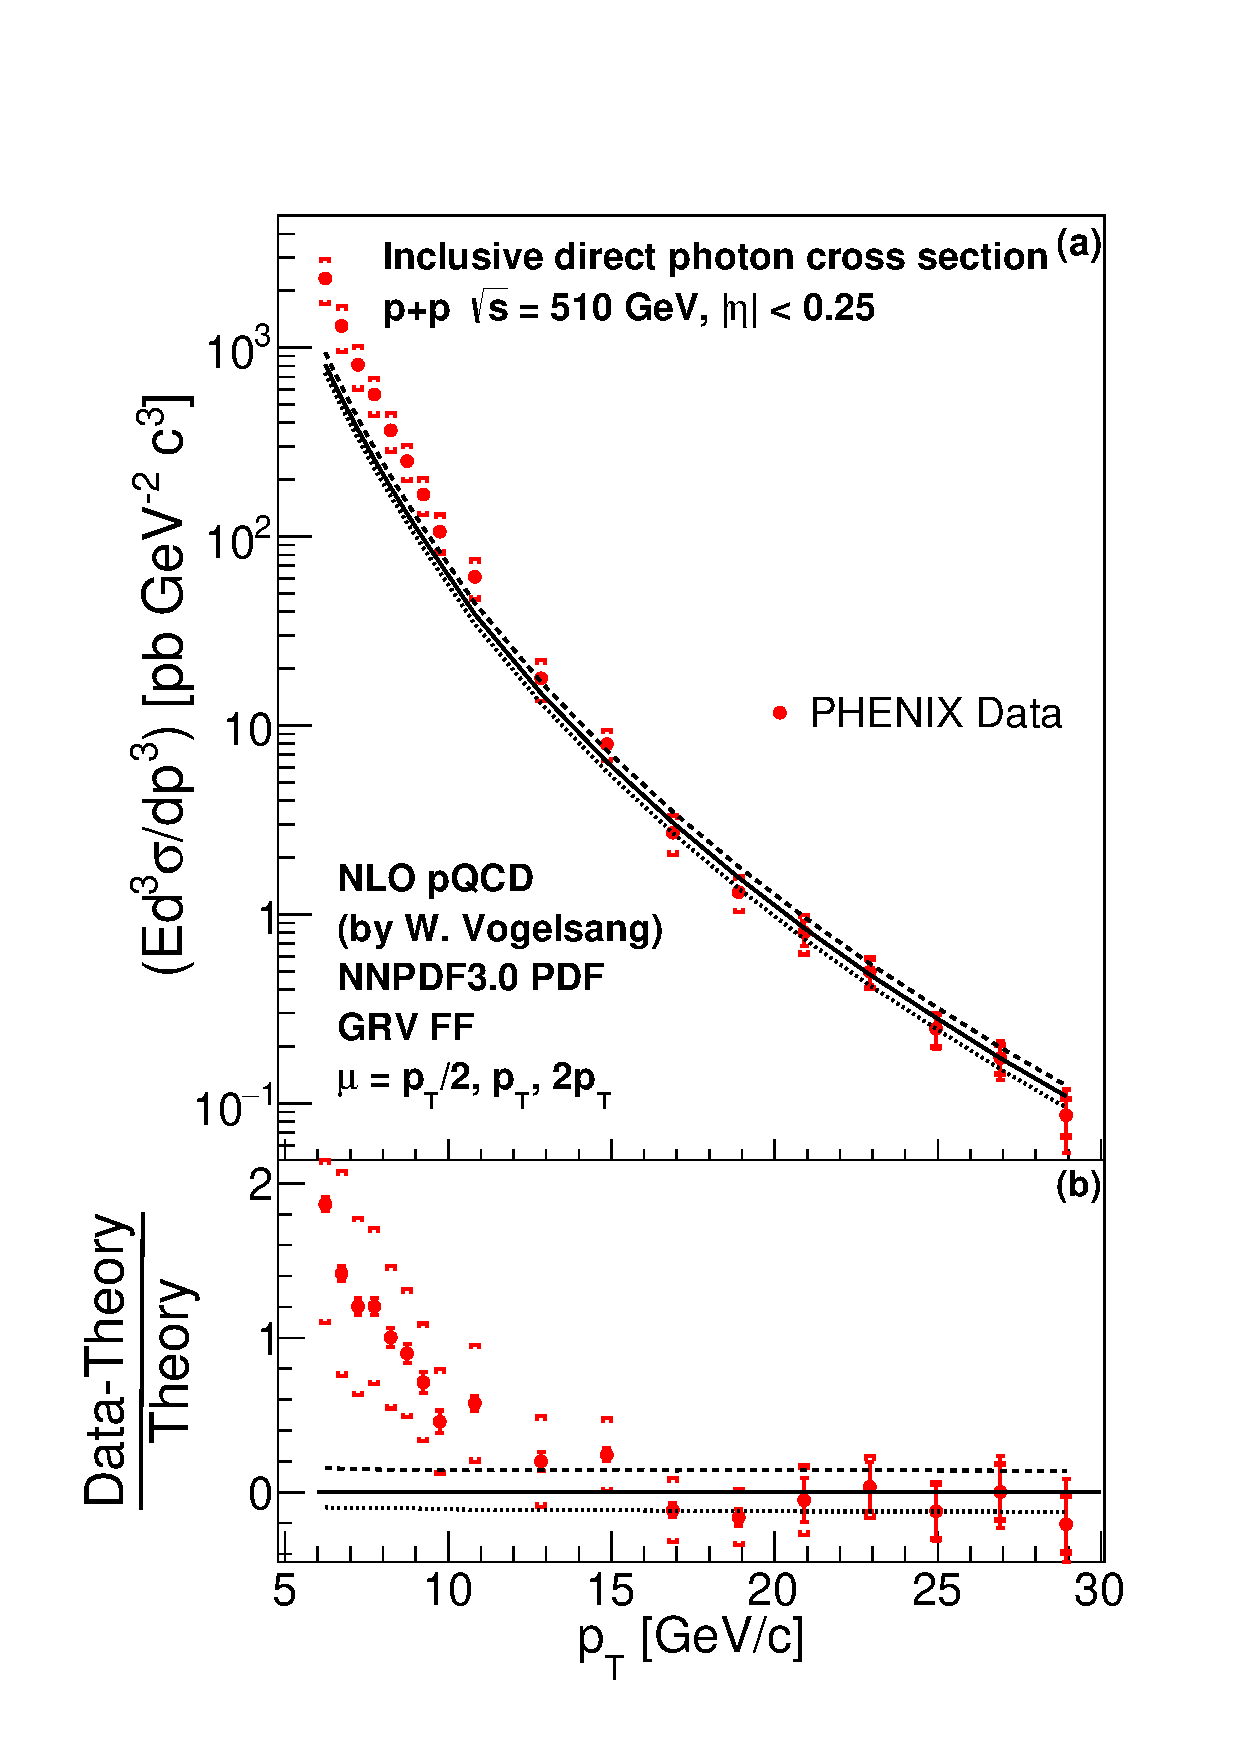
\includegraphics[width=0.5\textwidth]{CrossSection-photon-werner}
\caption{Inclusive direct photon cross section as a function of \pT\ compared with NLO pQCD calculations \cite{PhysRevD.48.3136,PhysRevD.50.1901} for different renormalization and factorization scales $\mu$ = \pT/2 (dashed line), \pT\ (solid line), 2\pT\ (dotted line). The bars represent statistical uncertainties and square brackets are for systematic uncertainties. The bottom plot shows the comparison of data and calculations.}
\label{fig:inc}
\end{figure}

%systematic here
The main systematic uncertainty sources are from global energy scale of tuning the \pizero\ mass peak position and energy nonlinearity of the EMCal response at high \pT, which are calculated by a single \pizero\ or photon generator with fast detector simulation and were determined to be between 14\% and 19\% depending on \pT. The systematic uncertainties due to \pizero\ yield extraction and relative fractions of other hadron decays over \pizero\ are 2-12\% and 5-14\%, respectively. The loss of photons from conversions in material before the EMCal is estimated using a single photon generator + GEANT full detector simulation \cite{Brun:1994aa}. The material of the vertex tracker \cite{SONDHEIM2012993} leads to a (12.8 $\pm$ 1.9)\% probability for a photon to convert. Since only West Arm has vertex tracker, this systematic uncertainty only influence direct photon yield from the West Arm. Conversions in other materials lead to (3 $\pm$ 1)\% in PbSc and (4.5 $\pm$ 1.3)\% in PbGl for photon loss. When calculating the direct photon yield in eq.~\ref{eq:inc} and eq.~\ref{eq:iso}, we vary the photon conversion rate by its systematic uncertainty to get 1-8\% relative uncertainties of direct photon yield. The uncertainties from EMCal detector resolution (2-8\%) and trigger (2-4.5\%) are also taken into account. Other uncertainties include geometrical acceptance, trigger efficiencies and pile-up effect and are in total less than 7\%.

The isolated direct photon cross section is shown in Fig.~\ref{fig:iso} as a function \pT\ and compared with the NLO pQCD calculation \cite{PhysRevD.48.3136,PhysRevD.50.1901} using NNPDF3.0 \cite{Ball2015,Bonvini2015} and GRV FF \cite{PhysRevD.45.3986}. The calculation is in good agreement with our data within the uncertainties. Similar to the inclusive cross section result, the global energy scale and energy nonlinearity are the major contributions to the systematic uncertainties, which are 7-13\% depending on \pT. The systematic uncertainties due to \pizero\ yield extraction and other hadrons' production ratio are 0.5-2.5\% and 0.4-6\%, respectively. These contributions are relatively smaller than the inclusive case as the isolation requirement largely reduces these backgrounds.

\begin{figure} 
\centering
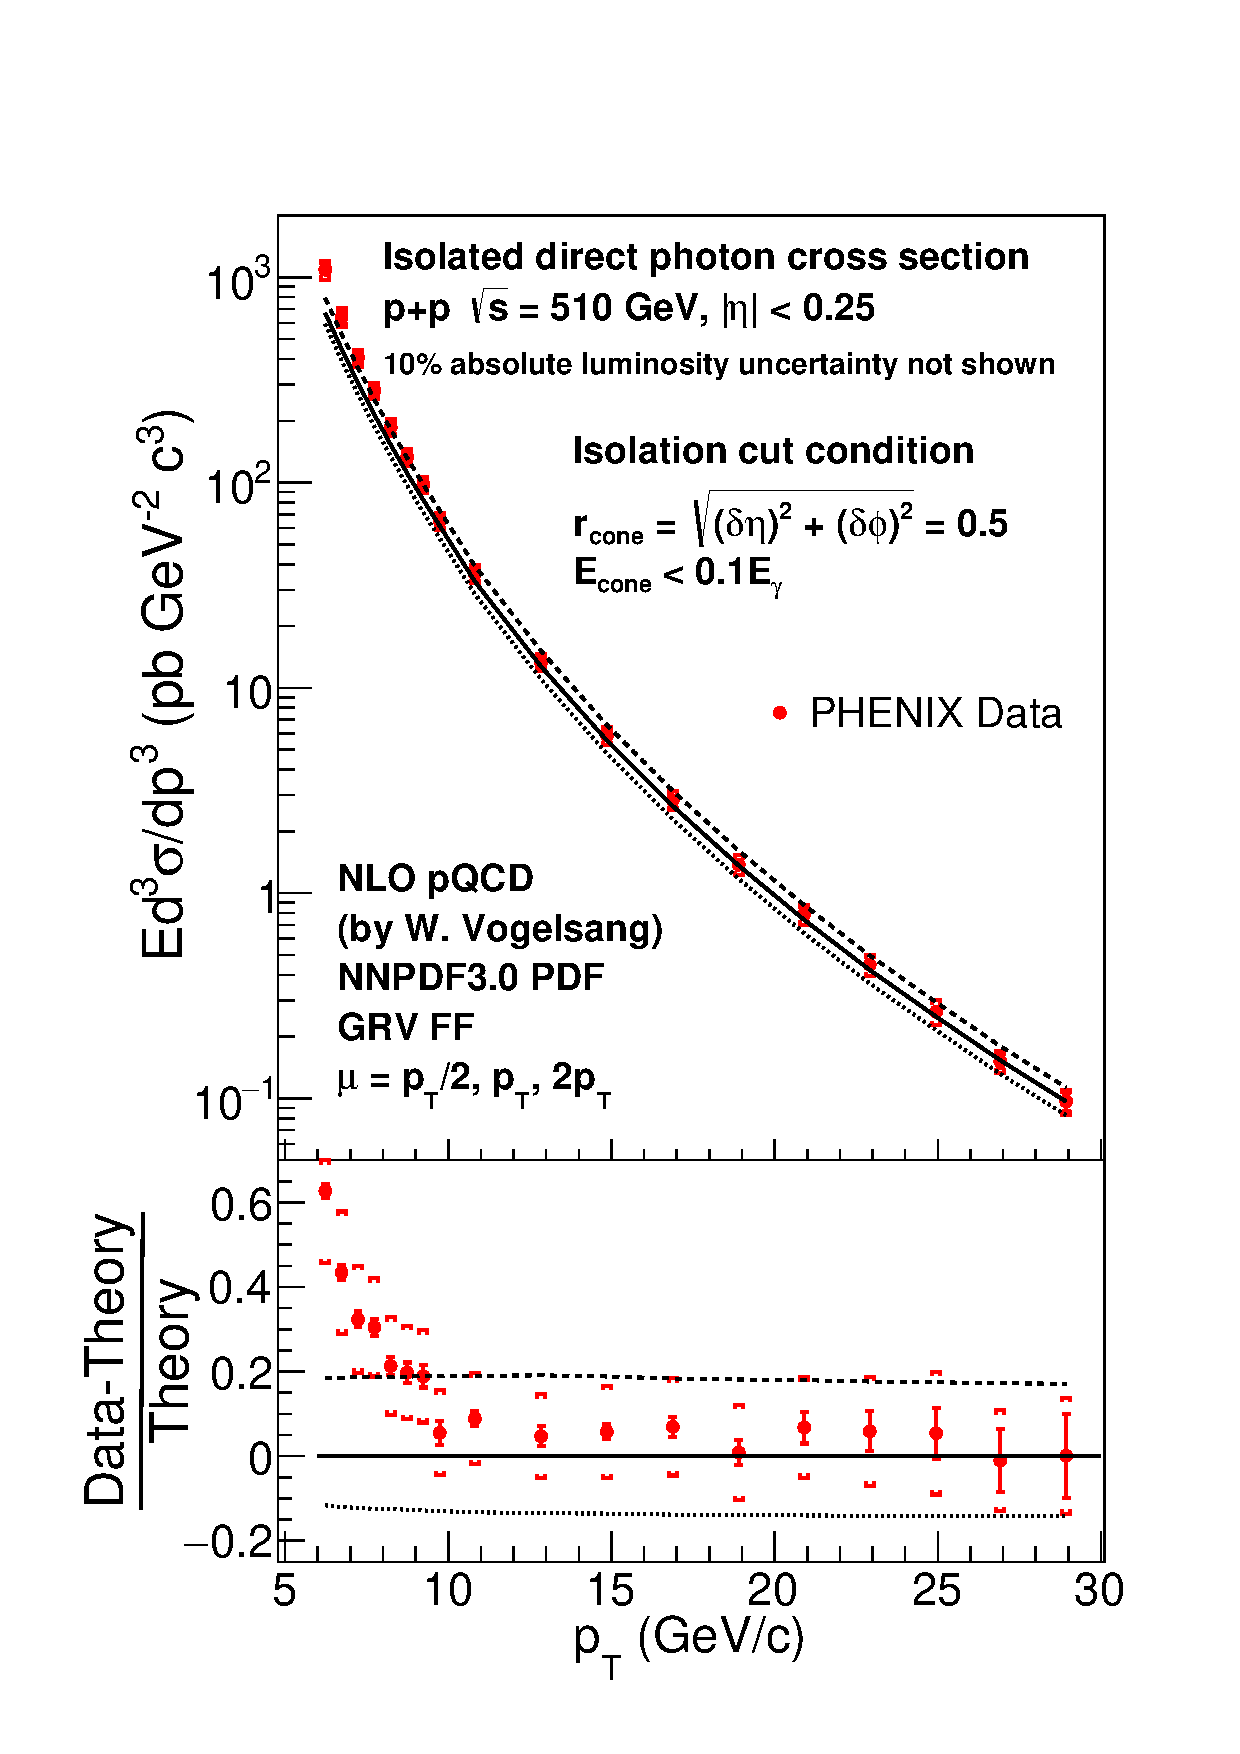
\includegraphics[width=0.5\textwidth]{CrossSection-isophoton-werner}
\caption{Isolated direct photon cross section as a function of \pT\ compared with NLO pQCD calculations \cite{PhysRevD.48.3136,PhysRevD.50.1901} for different renormalization and factorization scales $\mu$ = \pT/2 (dashed line), \pT\ (solid line), 2\pT\ (dotted line). The bars represent statistical uncertainties and square brackets are for systematic uncertainties. The bottom plot shows the comparison of data and calculations.}
\label{fig:iso}
\end{figure}

In Fig.~\ref{fig:iso2inc}, the ratio of isolated over inclusive direct photons is shown together with theoretical calculations. The MC simulations are from POWHEG + PYTHIA8 \cite{Nason_2004, Frixione_2007, Alioli2010, Jezo2016, Klasen2018}. POWHEG is a NLO partonic level generator, the output of which can be used as the input for PYTHIA8. The latter includes the multiparton interactions (MPI), parton showers (PS) and fragmentation processes. There is some phase space overlapping between POWHEG and PYTHIA8, which is solved by a proper veto algorithm. POWHEG uses CT14 parton distribution functions (PDF) \cite{PhysRevD.93.033006}. There is no final-state factorization scale in PYTHIA8 as it uses string fragmentation instead. In the POWHEG+PYTHIA8 simulations, the uncertainties from renormalization and factorization scales are canceled between the numerator and denominator of the fraction. The MC simulations were produced with and without MPI. When MPI is not included it overestimates the ratio similar to the NLO pQCD calculations while including MPI shows better agreement with this measurement.

\begin{figure}
\centering
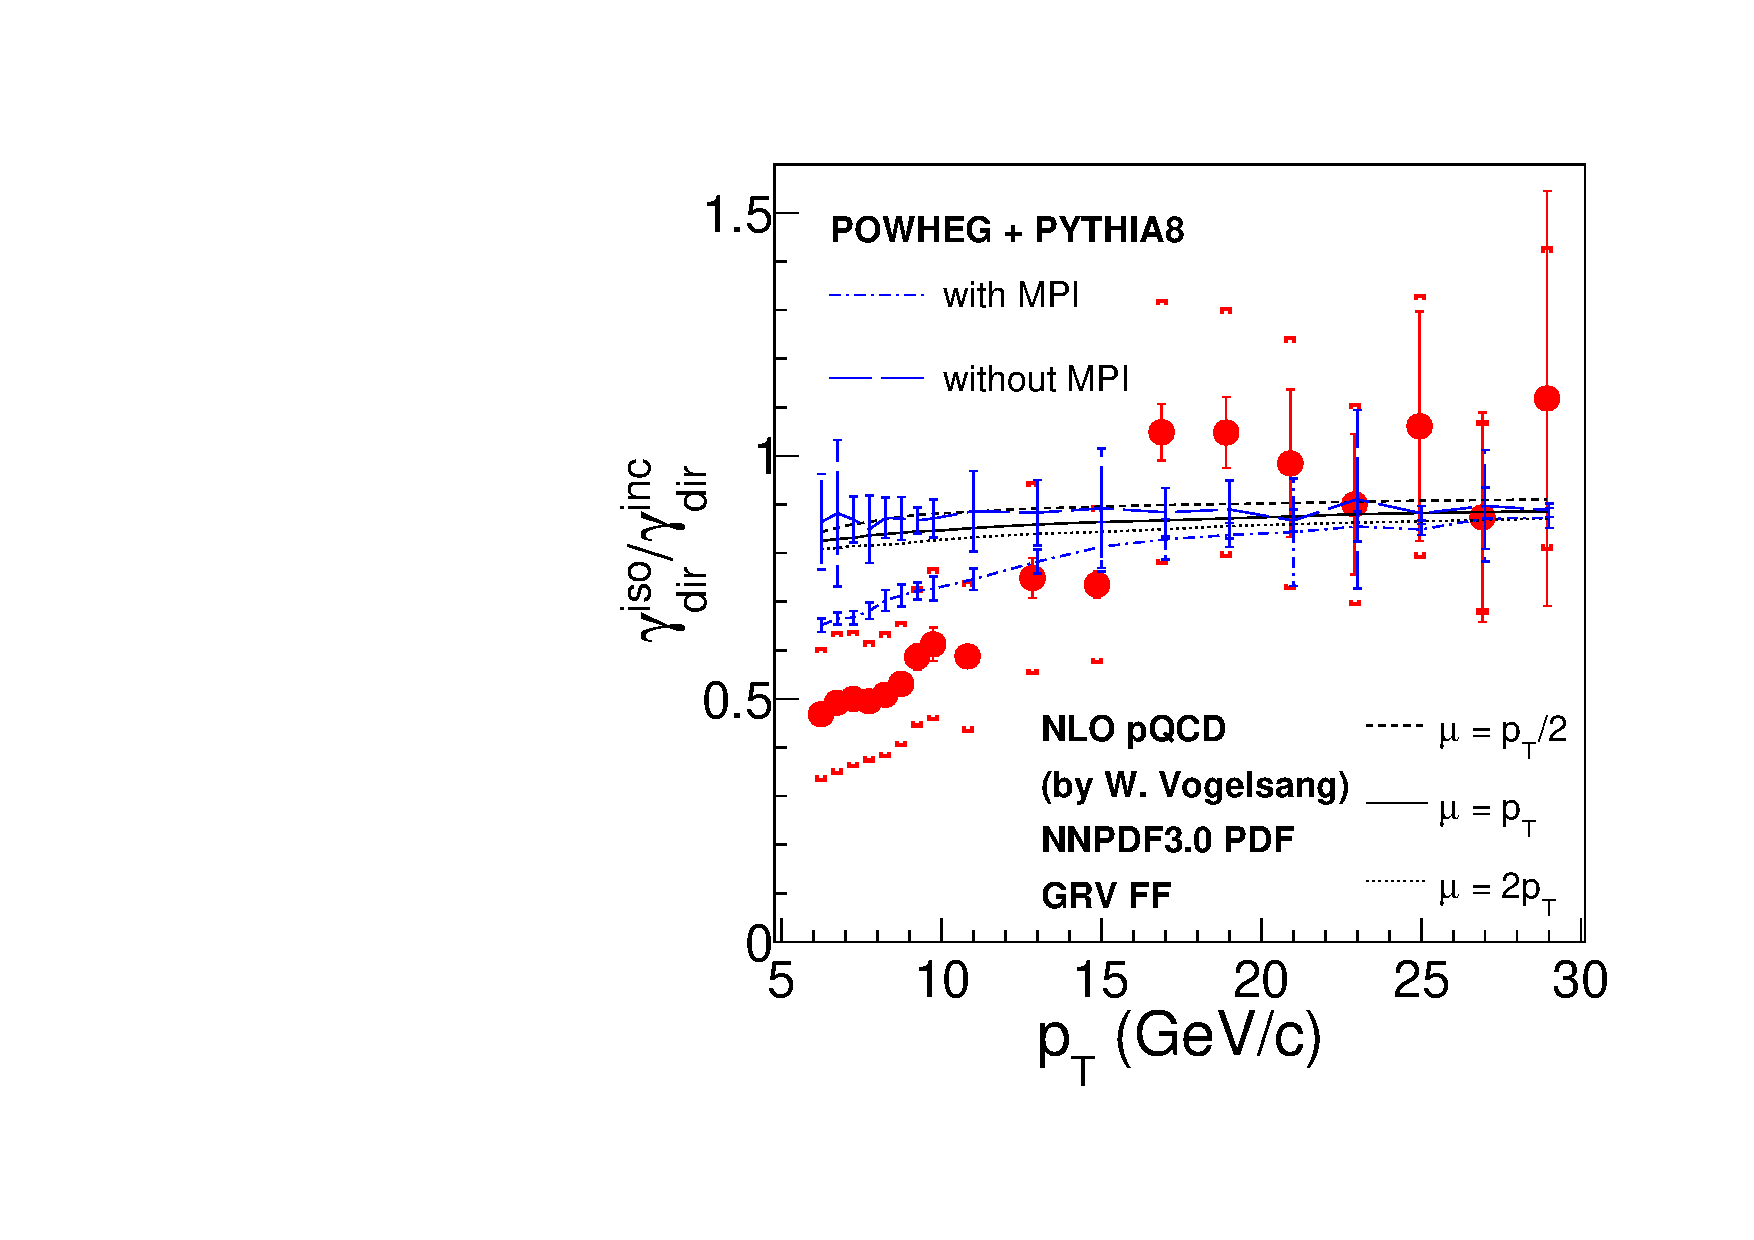
\includegraphics[width=0.5\textwidth]{Iso2Inc}
\caption{Isolated over inclusive direct photon ratio: bars are statistical uncertainties and square brackets are systematic uncertainties. POWHEG + PYTHIA8 without MPI and NLO pQCD calculations with different renormalization and factorization scales are also shown.}
\label{fig:iso2inc}
\end{figure}

The double helicity asymmetry is defined as

\begin{equation} \label{eq:all}
A_{LL} = \frac{\Delta\sigma}{\sigma} = \frac{\sigma_{++}-\sigma_{+-}}{\sigma_{++}+\sigma_{+-}},
\end{equation}
where $\sigma_{++}$ ($\sigma_{+-}$) is the cross section for the same (opposite) helicity proton collisions. This can be rewritten in terms of particle yield and beam polarizations:

\begin{equation}
A_{LL} = \frac{1}{P_BP_Y} \frac{N_{++}-RN_{+-}}{N_{++}+RN_{+-}}
\end{equation}
where $N_{++}$ ($N_{+-}$) is the number of isolated direct photons from the bunches with the same (opposite) helicities. $P_{B}$ and $P_{Y}$ are the polarizations for the two proton beams, and the average values in 2013 were 0.55 and 0.57, respectively \cite{POBLAGUEV2020164261}. $R$ $(= \mathcal{L_{++}}/\mathcal{L_{+-}}$) is the relative luminosity that is measured by the BBC. The systematic contribution of R to $A_{LL}$ was found to be 3.9 $\times$ $10^{-4}$.

The asymmetry was calculated for photon candidates that passed the same time-of-flight, minimum energy, and isolation requirements as the cross section analysis. The z-vertex requirement of 30 cm is used for the asymmetry measurement. The asymmetry contribution for background photons from \pizero's decay was calculated from the sideband region (47-97 MeV/$c^2$ and 177-227 MeV/$c^2$) around the \pizero\ mass peak (112-162 MeV/$c^2$) using the inclusive photon sample due to the limited statistics in the isolated photon sample. The asymmetry for other hadron decays (mostly $\eta$'s decay) was taken as $A_{LL}^{\eta}$ from previous PHENIX measurement at $\sqrt{s}$ = 200 GeV \cite{PhysRevD.90.012007} by assuming $x_T$ scaling. The difference in $A^{\eta}_{LL}$ between 200 GeV and 510 GeV for a given $x_{_{T}}$ is expected to be much smaller than the experimental uncertainty of the 200 GeV result which was used to assign a systematic uncertainty \cite{PhysRevLett.113.012001, 2014276}. The background corrected asymmetry can be calculated as

\begin{equation} \label{eq:all-dir}
A_{LL}^{dir} = \frac{A_{LL}^{total} - r_{\pi^0}A_{LL}^{\pi^0} -r_h A_{LL}^{\eta}}{1 - r_{\pi^0} - r_h},
\end{equation}
where $r_{\pi^0}$ (10-14\%) and $r_h$ (0.6-1.4\%) are background fractions of \pizero\ and other hadron decay photons, respectively. Consistency checks of asymmetries were performed to ensure that there is no hidden systematic effect and the asymmetry is calculated reliably. The data were divided into subgroups according to the bunch spin patterns that were used to fill the RHIC rings, and calculated asymmetries were found to be consistent.

\begin{figure}[htb]
\centering
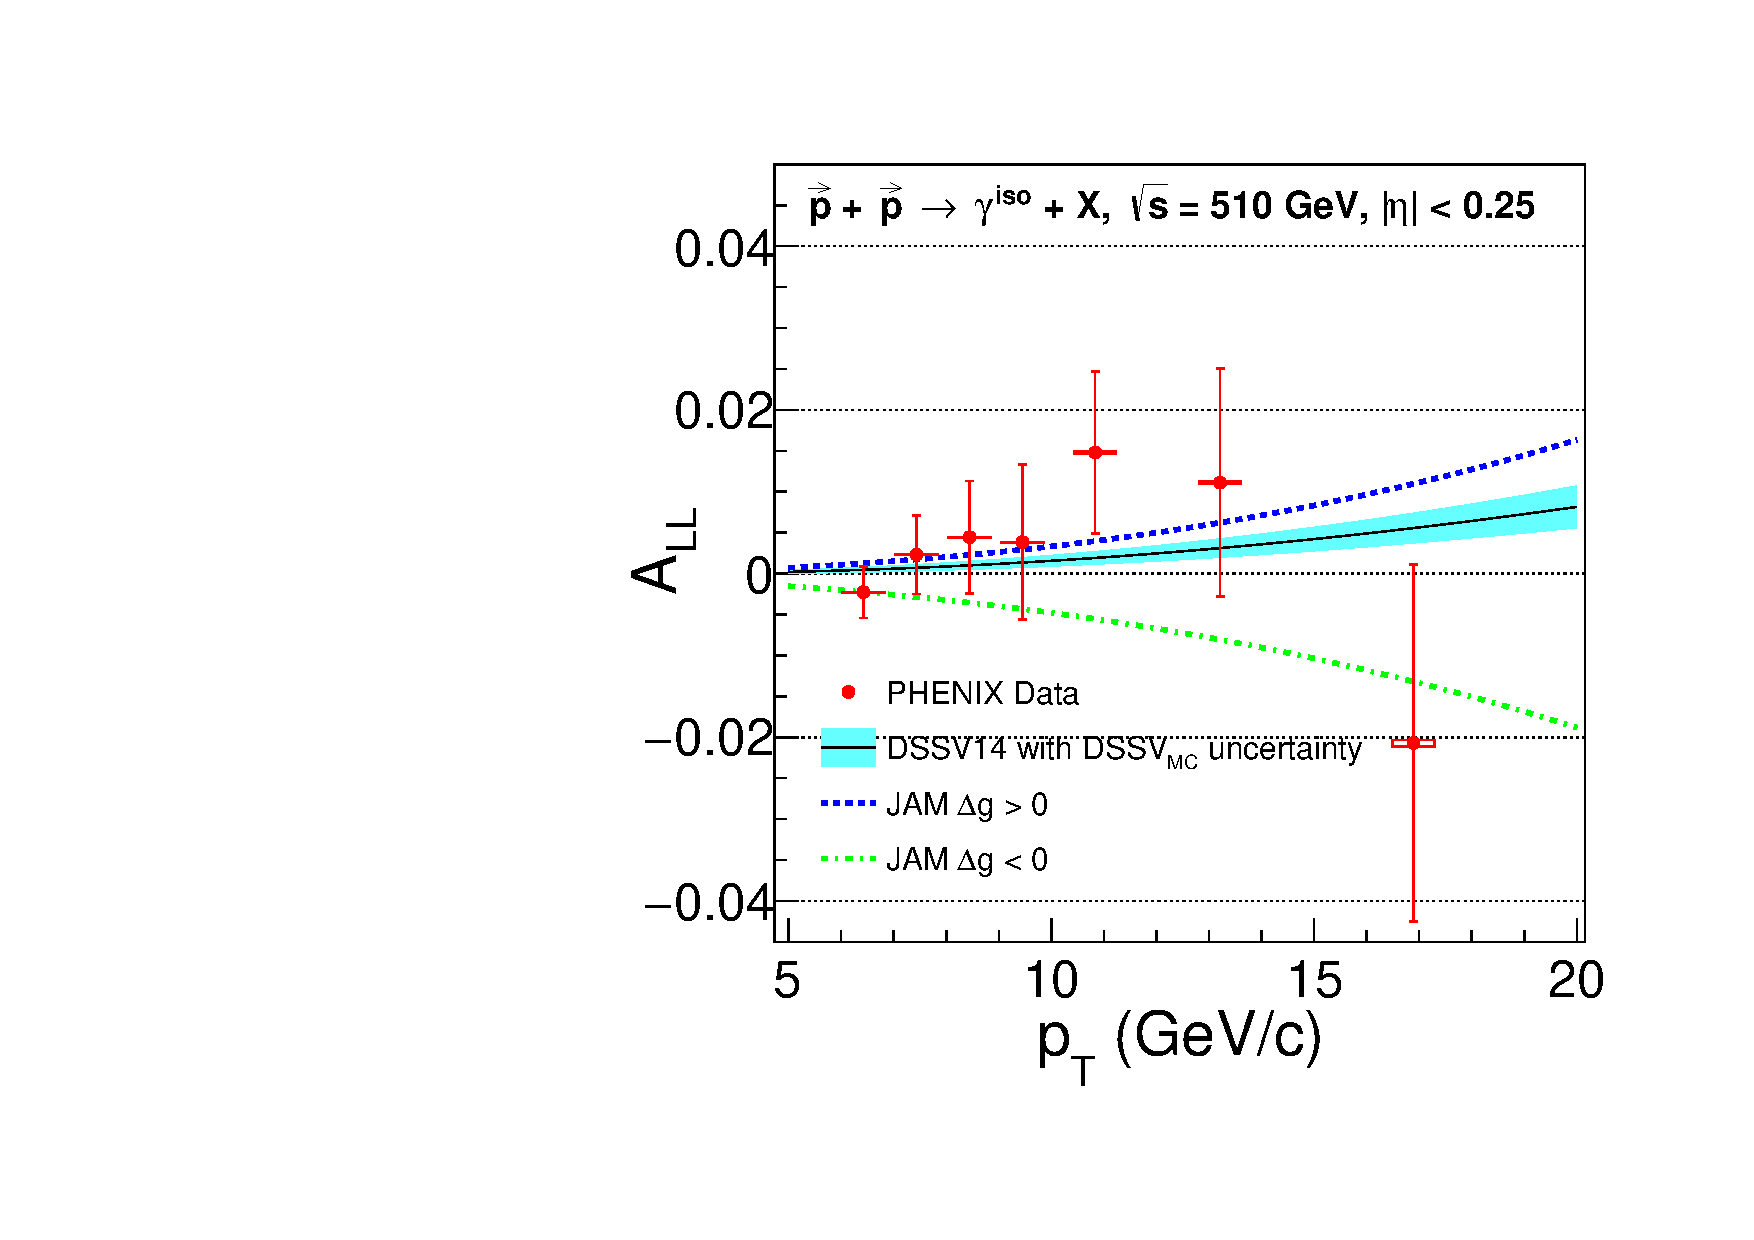
\includegraphics[width=0.5\textwidth]{IsoPhotonALL-beam2}
\caption{Double helicity asymmetry $A_{LL}$ $vs$ $p_{T}$ for isolated direct photon production in polarized p+p collisions at $\sqrt{s}$ = 510 GeV at midrapidity. Vertical error bars (boxes) represent the staistical (systematic) uncertainties. The NLO pQCD calculation is plotted as the solid curve with $1\sigma$ uncertainty band from MC replica \cite{PhysRevLett.101.072001,PhysRevLett.113.012001,PhysRevD.100.114027}.}
\label{fig:all}
\end{figure}

The double helicity asymmetry of isolated direct photon production in longitudinally polarized proton collisions at $\sqrt{s}$ = 510 GeV is shown in Fig.~\ref{fig:all} for 6 $< p_{T} <$ 20 GeV/c. The NLO pQCD calculation was obtained using DSSV14 polarized PDF, NNPDF3.0 unpolarized PDF and GRV FF for the renormalization and factorization scales $\mu = p_T$ with $1\sigma$ uncertainty band from MC replicas \cite{PhysRevLett.101.072001,PhysRevLett.113.012001,PhysRevD.100.114027}. The calculation is in good agreement with our results within the experimental uncertainties. In the asymmetry measurement systematic effects are largely canceled. The systematic uncertainties in Fig.~\ref{fig:all} include point-to-point uncertainties from background estimation and false asymmetry in background due to pile-up effect at low \pT.

In summary, PHENIX has measured the cross section and \ALL\ of direct photon at midrapidity in proton collisions at $\sqrt{s}$ = 510 GeV. The NLO pQCD calculations are overall consistent with our results except at lower \pT\ where the calculations underestimate the cross section. The calculations including underlying events such as MPI and PS give a better description for the isolated over inclusive cross section ratio which indicates the importance of considering such contributions to understand the results at low $p_{T}$. It is the first time that the \ALL\ of direct photon is measured. This is sensitive to the polarized gluon distribution inside the proton and will provide an independent constraint on the gluon spin contribution to the proton spin when included in the future global analyses.
%%% For help see /phenix/WWW/p/info/dp/000/template/template4.tex

%%% To check PRL length insert these (uncommented) lines here:
\clearpage \textbf{*** page break for PRL word count $<$3.5 pages $<$7 columns ***}

%%%%%%%%%%%%%%%%%%%%%%%%%  Acknowledgements 
% for PRC or PRD only, uncomment this line:
%\section*{ACKNOWLEDGMENTS}  

%% Acknowledgments are determined by runs for which new results are
%% being released.  As with the author lists, Brant will add later
%% by using the most current acknowledgments, plus any additions
%% from relevant runs.  For example, new Run-6 releases include:
%% "a sponsored research grant from Renaissance Technologies LLC,"

%%%%%%%%%%%%%%%%%%%%%%%%%%%  References 

\bibliography{references}   % Use of BibTeX required.

\end{document}